
% ********** Chapter 7 **********
\chapter{Web Application}
\label{sec:WebApplication}

\section{Overview}
\label{sec:WebApplication:Overview}

\begin{figure}[!hbtp]
\centering
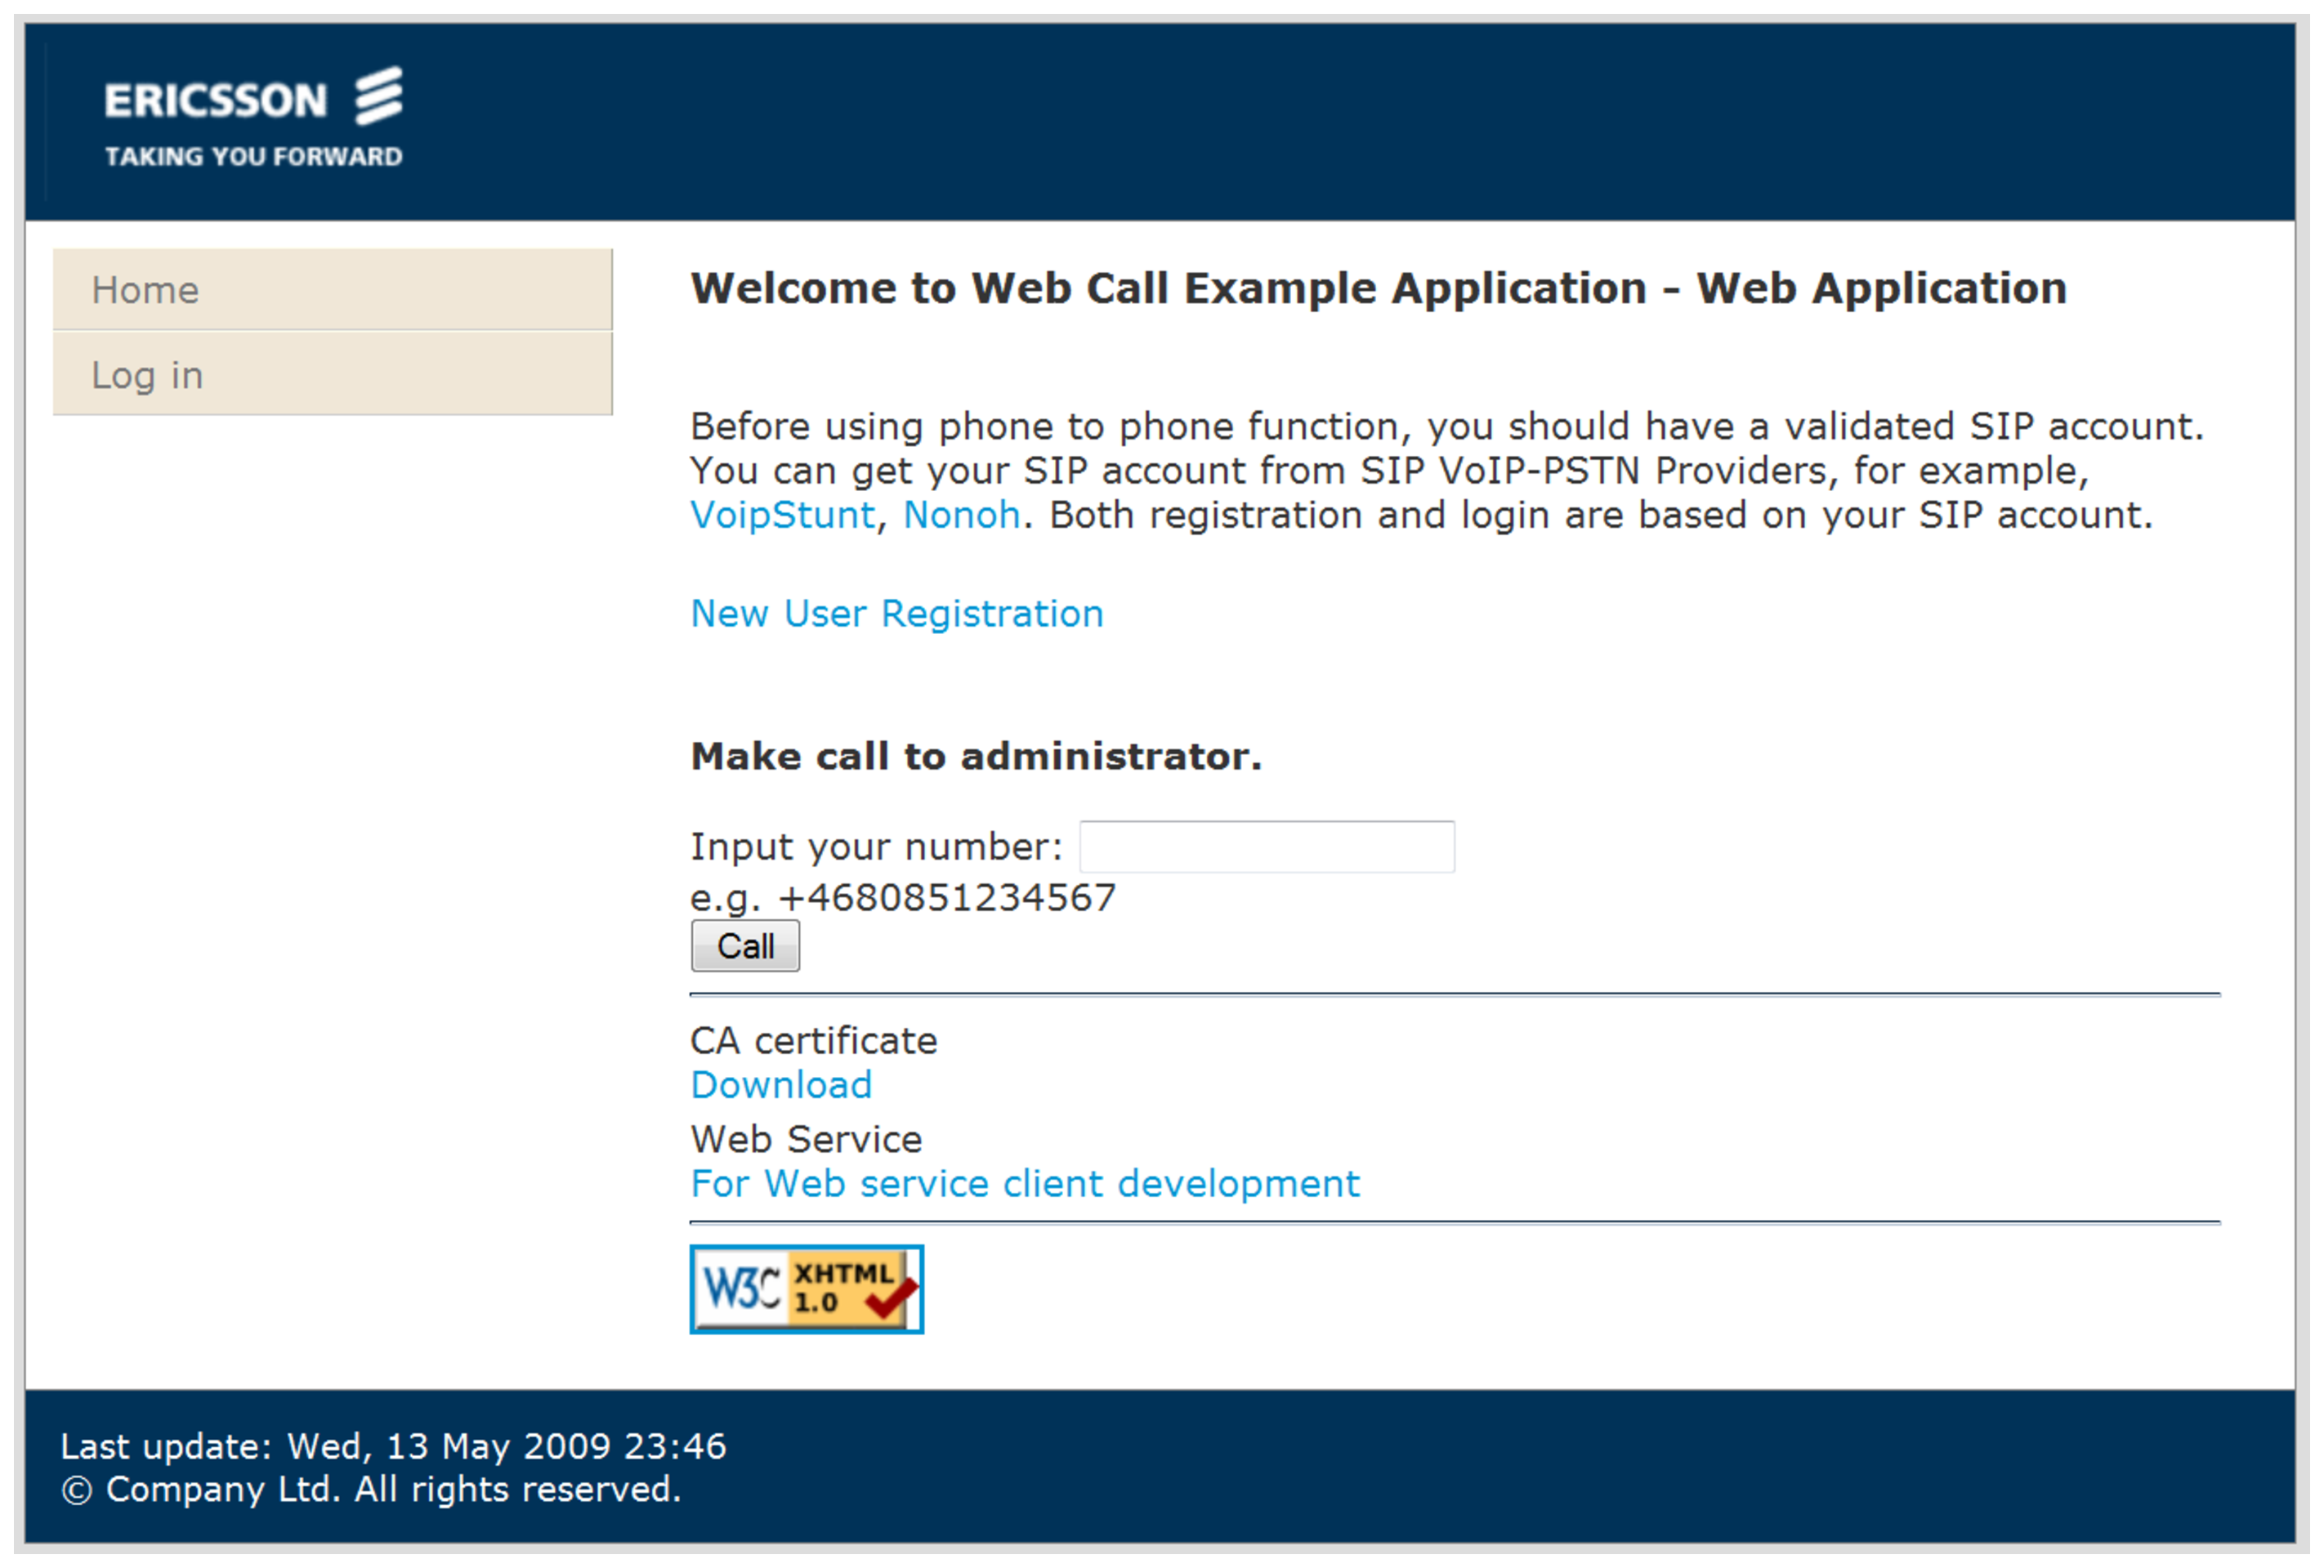
\epsfig{file=chap07/resources/welcome_desktop_browser_view, width=5.2in}
\caption{Welcome page of desktop browser view of web application}
\label{fig:WelcomePageOfDesktopBrowserView}
\end{figure}

The web application is the main portal of the whole application. It is based on Mobile Front Controller. The role of web application in the whole application is shown in Figure \ref{fig:ArchitectureOfWebCallSDK}. Users can use the web application to manage their accounts and VoIP calls. Administrators can use web applications to manage users. The web application can be packaged into a war file and easily to deploy. It only needs a sevlet container, like Tomcat, to run. It supplies two kind of views one is for desktop browser and another is for mobile browser. Beside these two views, the web application also contains a web service interface. This chapter will focus on two browser view. The web service interface will be introduced with detail in chapter \ref{sec:WebServiceInterface}.

A welcome screen of desktop browser view of Web Application is shown in Figure \ref{fig:WelcomePageOfDesktopBrowserView}.

\section{Architecture of Mobile Front Controller 3}
\label{sec:WebApplication:ArchitectureOfMobileFrontController3}

\textit{``Mobile Front Controller (MFC)\label{sym:MFC} is a light-weight Java EE web application framework for creating web applications for web browsing and mobile browsing.''}\cite{MobileFrontController} It was developed by Peter Yeung and P\"{a}r Johansson from \href{http://www.ericsson.com/developer/}{Ericsson Developer Connection}, Ericsson\cite{MobileFrontController}. The mobile front controller uses a sevlet to handle http request, and redirect request to different kind of view. All views share a same logic. An overview of Mobile Front Controller used by a web application on a Java EE web container is shown in Figure \ref{fig:MFCOverview}.

\begin{figure}[!hbtp]
\centering
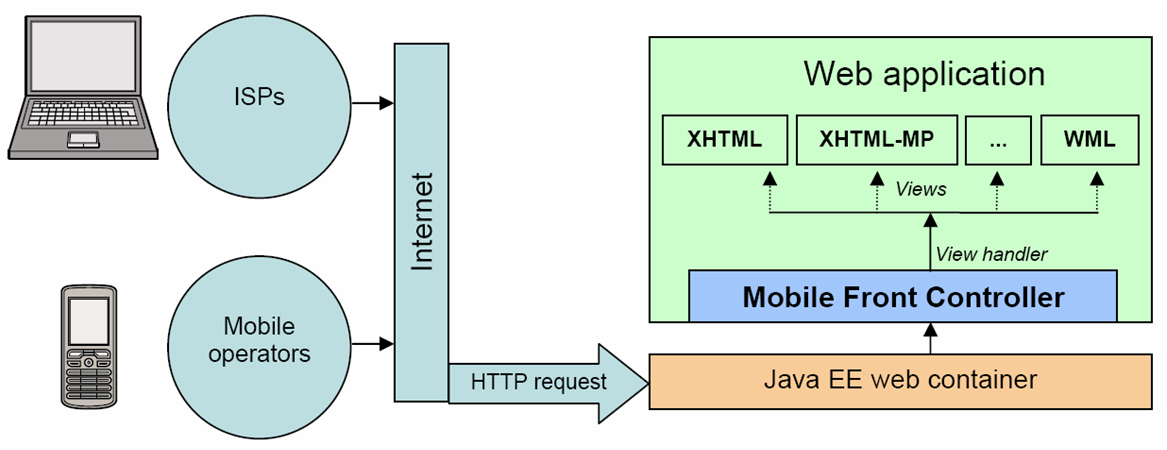
\epsfig{file=chap07/resources/MFC_overview, width=5.2in}
\caption{An overview of Mobile Front Controller used by a web application on a
Java EE web container. (Figure taken from \textit{Mobile Front Controller Developer's guide for software version 3.1}\cite{DevelopersGuideOfMFC})}
\label{fig:MFCOverview}
\end{figure} 

\textit{``MFC is used on top of a Java EE web container, and does not require any other framework, such as JSF, Struts, etc.
MFC does the following:}
\begin{itemize}
\item \textit{{Detects and selects appropriate views based on HTTP request headers. A view is a subdirectory that, for example, corresponds to a markup language such as XHTML, XHTML Mobile Profile (MP) and WML (see Figure \ref{fig:ArchitecureOfMFC}). The way MFC detects and selects views is customizable using view handlers.} }
\item \textit{Shares UI logic between different views, for example, web and mobile browsing. This is done using action commands, which are classes that contain an execute method that is executed when a URL with, for example, the URL pattern *.do is called (for example http://localhost:8080/mfc-basic-demo/xhtml/Print.do).''}\cite{DevelopersGuideOfMFC}
\end{itemize}

\begin{figure}[!hbtp]
\centering
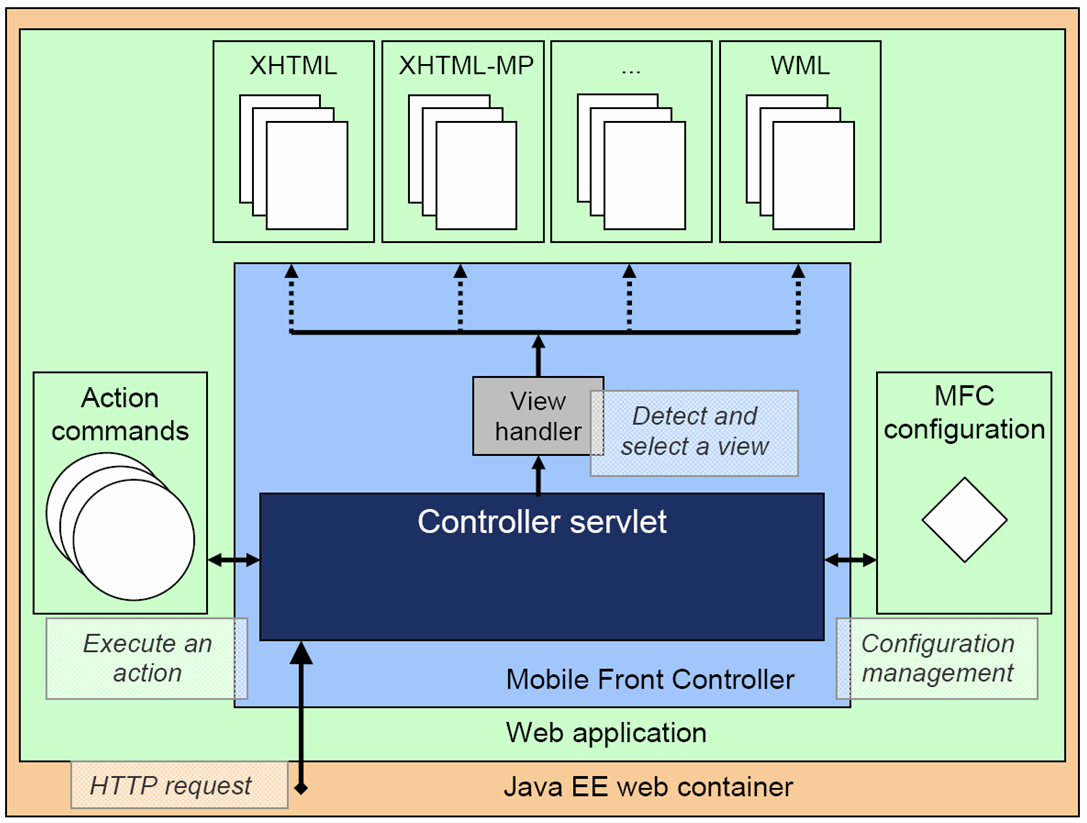
\epsfig{file=chap07/resources/architecture_of_mfc, width=5.2in}
\caption{The architecture of Mobile Front Controller (Figure taken from \textit{Mobile Front Controller Developer's guide for software version 3.1}\cite{DevelopersGuideOfMFC})}
\label{fig:ArchitecureOfMFC}
\end{figure} 

The version of Mobile Front Controller used in Web Call Example Application is the latest version, v3.1.

\section{Dual view}
\label{sec:WebApplication:DualView}

As described in the section \ref{sec:WebApplication:ArchitectureOfMobileFrontController3}, Mobile Front Controller supplies multi-view function. Web Call Example Application is developed with two view, one is desktop browser view and the other is mobile browser view. The will be illustrated separately in subsection \ref{sec:WebApplication:DualView:DesktopBrowserView} and \ref{sec:WebApplication:DualView:MobileBrowserView}.

\subsection{Desktop browser view}
\label{sec:WebApplication:DualView:DesktopBrowserView}

The Mobile Front Controller supplies a function of select view. If the user access web application via a desktop browser, the desktop browser view (XHTML view) will return to user. The desktop browser view is a normal web site that follows the standard of The XHTML 1.0. Extensible HyperText Markup Language (XHTML\label{sym:XHTML}) is a markup language for web pages which developed by W3C HTML Working Group. It is widely used as a standard language of web page on Internet. A example page (welcome page) of desktop browser view is shown in Figure \ref{fig:WelcomePageOfDesktopBrowserView}.

\subsection{Mobile browser view}
\label{sec:WebApplication:DualView:MobileBrowserView}

If the user access web application via a mobile browser, the mobile browser view (XHTML MP view) will return to user. The mobile browser view is a normal web site that follows the standard of XHTML MP 1.1. XHTML Mobile Profile (XHTML MP) is a computer language standard designed specifically for mobile phones. It is developed by  A example page (welcome page) of mobile browser view is shown in Figure \ref{fig:WelcomePageOfMobileBrowserview}.

\begin{figure}[!hbtp]
\centering
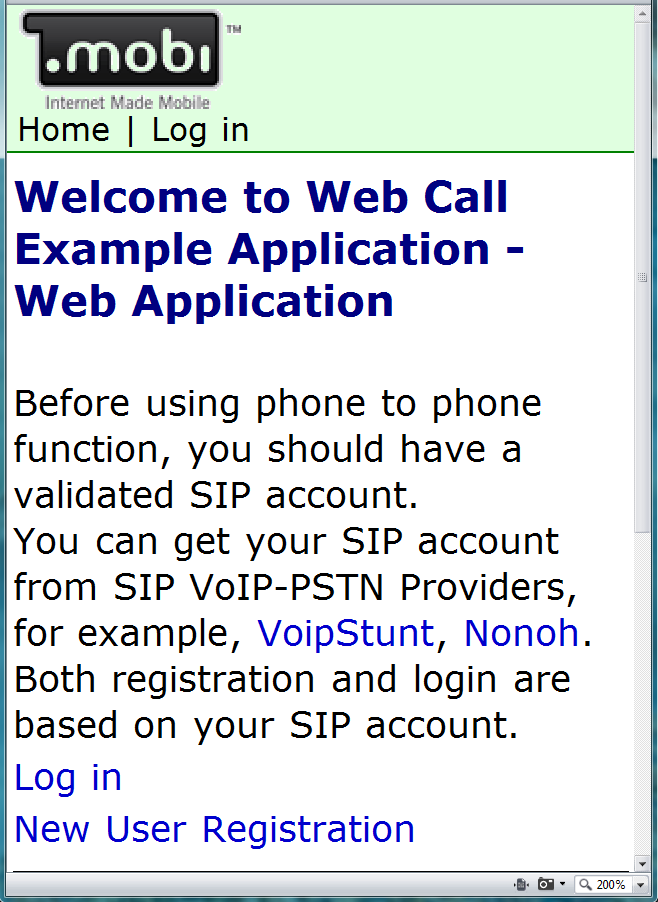
\epsfig{file=chap07/resources/welcome_mobile_view, width=2.5in}
\caption{Welcome page of mobile browser view}
\label{fig:WelcomePageOfMobileBrowserview}
\end{figure} 

\section{Site structure}
\label{sec:WebApplication:SiteStructure}

The web set structure contains three levels. \texttt{Base} \textrightarrow{} \texttt{Protected} \textrightarrow{} \texttt{admin}. Both desktop browser view and mobile browser view use the exactly same structure. 

Under base directory, there is welcome page, user register page and login page. The pages on this level are public opened. There are no restrictions on requesting these pages. 

All pages in protected directory are authenticated resources. To visit these pages, the user has to login first. Both user and administrator can request this kind of resources. Under user panel, user can freely edit information, e.g. user phone number, contact book, change password, VoIP provider account and recent calls. Users can make VoIP calls by clicking the link of Phone to Phone Call under user panel. 
The pages under admin directory are used for managing user information. Only user who has a role of administrator can access pages under admin directory. Administrator can modify user information or even delete users. 
For more details about security, please refer section \ref{sec:WebApplication:Security:SecurityConstraint}.

\section{User action}
\label{sec:WebApplication:UserAction}

\subsection{User Registration}

To use the Web Call Example Application, a user must register him on the web site. It is quite easy and simple to register and there are only three steps: 
\begin{enumerate}
\item Navigate to the web site url and open the welcome page. There are user registration functions on both desktop and mobile views. So users can register either from a computer or a mobile phone.
\item At the welcome page. Click the link to New User Registration.
\item Fill the form, include user name (in the format of email address), password and confirm password.
\end{enumerate}

\subsection{User panel}

The user profile information menu is shown in Figure \ref{fig:UserProfileInformationDesktopView}. User can edit his phone number, contact book, password, VoIP provider accounts and recent calls log.

\begin{figure}[!hbtp]
\centering
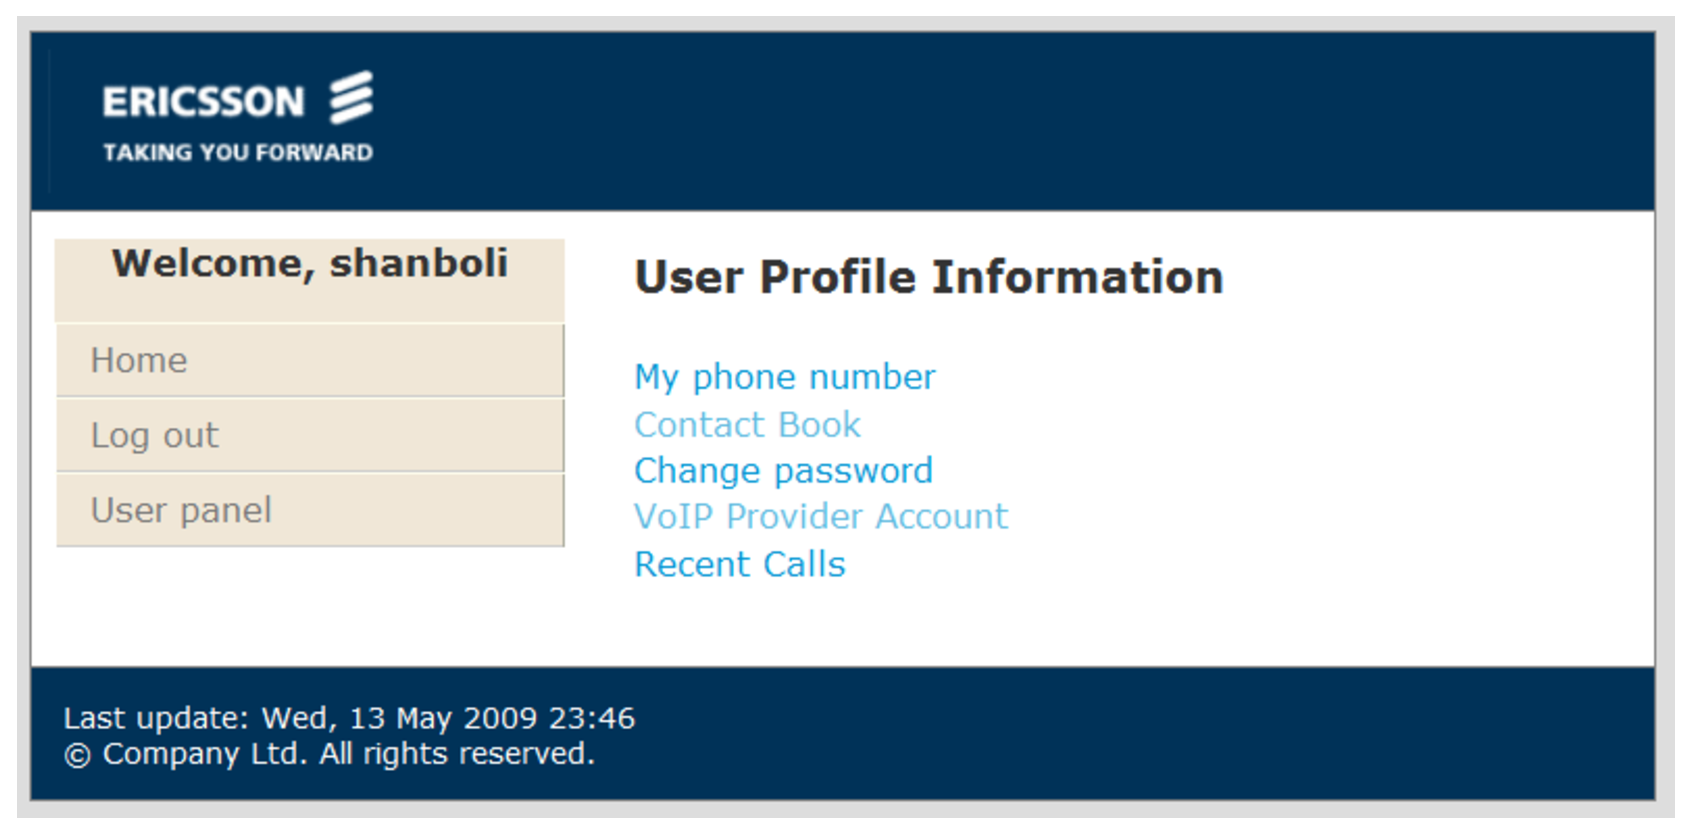
\epsfig{file=chap07/resources/user_profile_info_desktop_view, width=5.2in}
\caption{User profile information page of desktop browser view}
\label{fig:UserProfileInformationDesktopView}
\end{figure} 

\subsection{VoIP service provider account}

To make a VoIP call, the user must have a VoIP Provider Account first. Figure \ref{fig:RegisterVoIPAccount} shows how to register a VoIP provider account. To get the view of adding VoIP provider account, user should go to user panel \textrightarrow{} User Profile Information \textrightarrow{} VoIP Provider Account \textrightarrow{} add new VoIP provider account.
Follow the example in Figure \ref{fig:RegisterVoIPAccount} and input the VoIP account information. The outbound proxy should in a format of SIP\_PROVIDER\_URL:PORT\_NUMBER. If no port number specified, the port \texttt{5060} will be used as defined in RFC3261\cite{RFC3261}.

\begin{figure}[!hbtp]
\centering
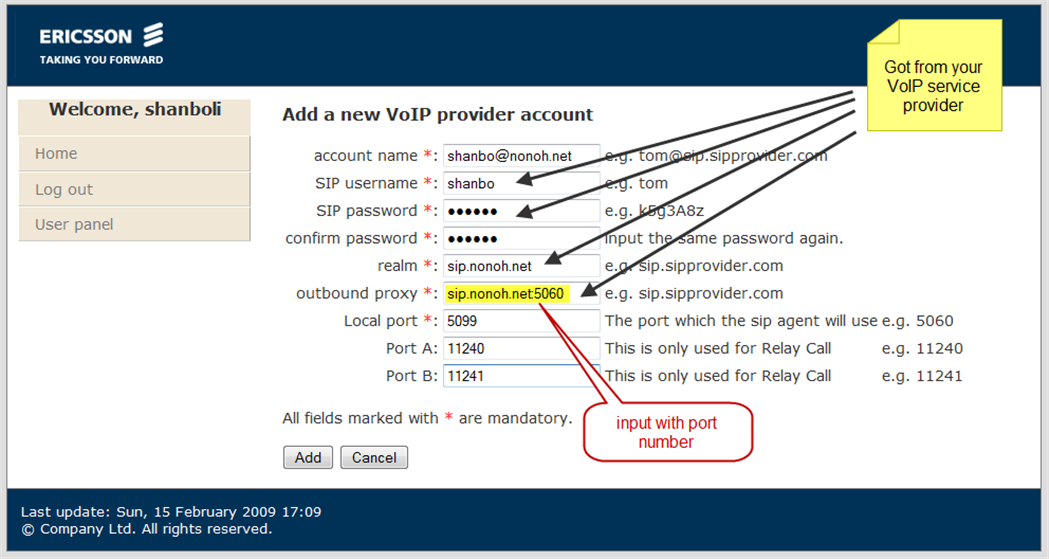
\epsfig{file=chap07/resources/register_voip_service_provider_account, width=5.2in}
\caption{Register VoIP service provider account}
\label{fig:RegisterVoIPAccount}
\end{figure} 

Web Call Example Application supports multi-account. This means as a user, you can have more than one account and choose a cheaper one when you make VoIP calls.

\subsection{Phone-to-Phone call}

The integrated web application offers phone-to-phone function for registered users. 

Figure \ref{fig:UserPanelDesktopBrowserView} is the user panel of desktop browser view. Users can either go to user profile Information page or the phone-to-phone dialing page. To make VoIP calls, the user just need click the link of Phone to phone call.

\begin{figure}[!hbtp]
\centering
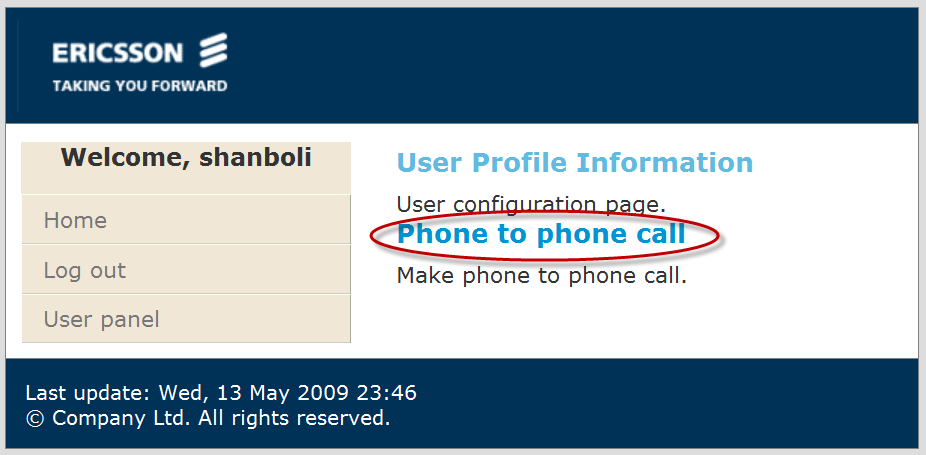
\epsfig{file=chap07/resources/user_panel_desktop, width=5.2in}
\caption{User panel desktop browser view}
\label{fig:UserPanelDesktopBrowserView}
\end{figure} 

\begin{figure}[!hbtp]
\centering
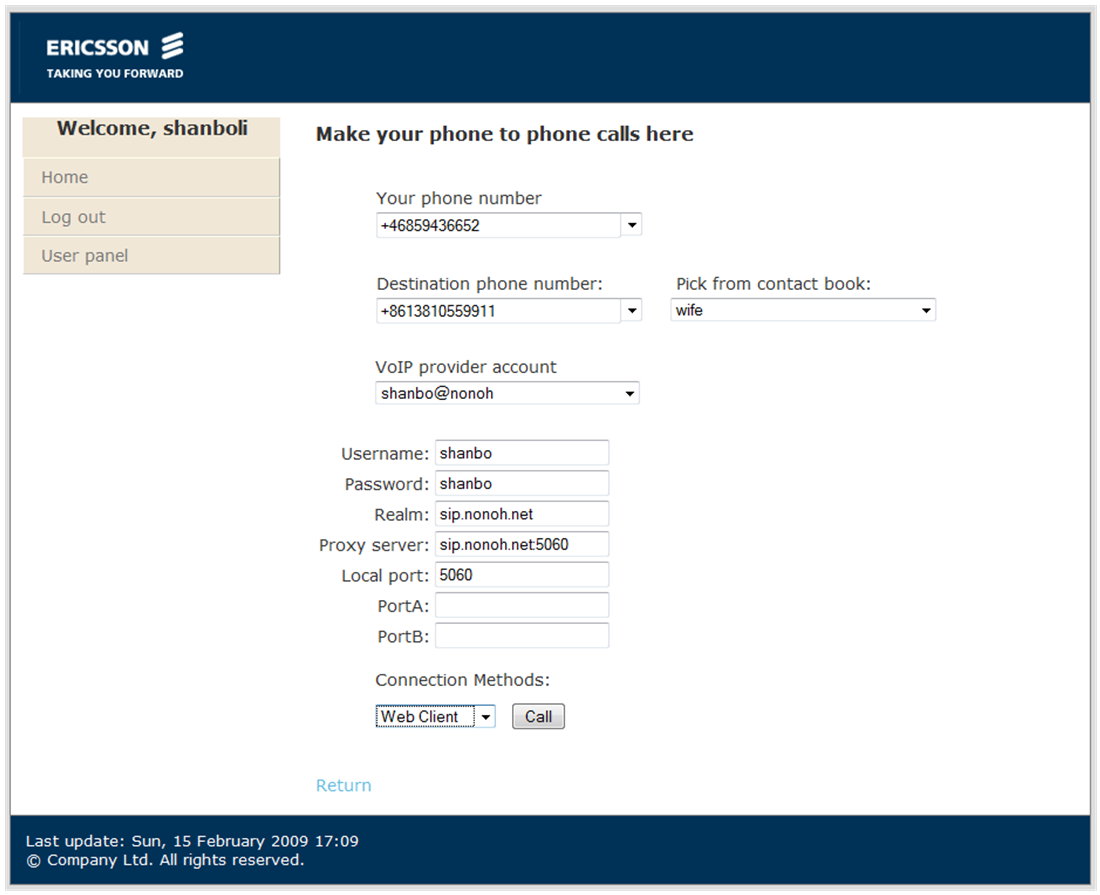
\epsfig{file=chap07/resources/phone_to_phone_call_desktop, width=5.2in}
\caption{Phone to phone call}
\label{fig:PhoneToPhoneCall}
\end{figure} 

In the phone-to-phone call page, which is shown in Figure \ref{fig:PhoneToPhoneCall}, users can input their own number, or use the default numbers, which is set in ``my phone number'' of user profiles information. And input the destination phone number, or select from recent calls or the contact list. The client number could either be SIP address or a complete phone number. If users have more than one VoIP provider account, they can use the drop down list of VoIP provider account and choose an account as their wish. Different VoIP service provider may supply different rate for different destination. So the multi-account function can help user save money by choosing a cheapest provider. This page uses the technology of Ajax to dynamically show the information of VoIP account. More Ajax technologies will be introduced in section \ref{sec:WebApplication:AjaxInWebApplication}. 

There is a drop down list of call methods. Five different implementations of connection methods will be illustrated at that list. They are Relay Call, Call transfer, Re-invite, SDP swap and Web client. The last four methods are so called third party call control (3PCC)\cite{RFC3725}. The differences of connection methods will be discussed in chapter \ref{sec:Solution}. It is recommend that by default user uses the method of Web client. 

After user clicked ``Call'' button. The page will be directed to call state page. On call state page, users can see the phone numbers of two sides, call state, or even cancel the call.

\section{Administrator action}
\label{sec:WebApplication:AdministratorAction}

The administrator actions include user profile management as well as all of user relevant information. 
Figure \ref{fig:UserListOfAdministratorPanel} is the user list page. The administrator can use the button of edit to change the user information as well as user roles.

\begin{figure}[!hbtp]
\centering
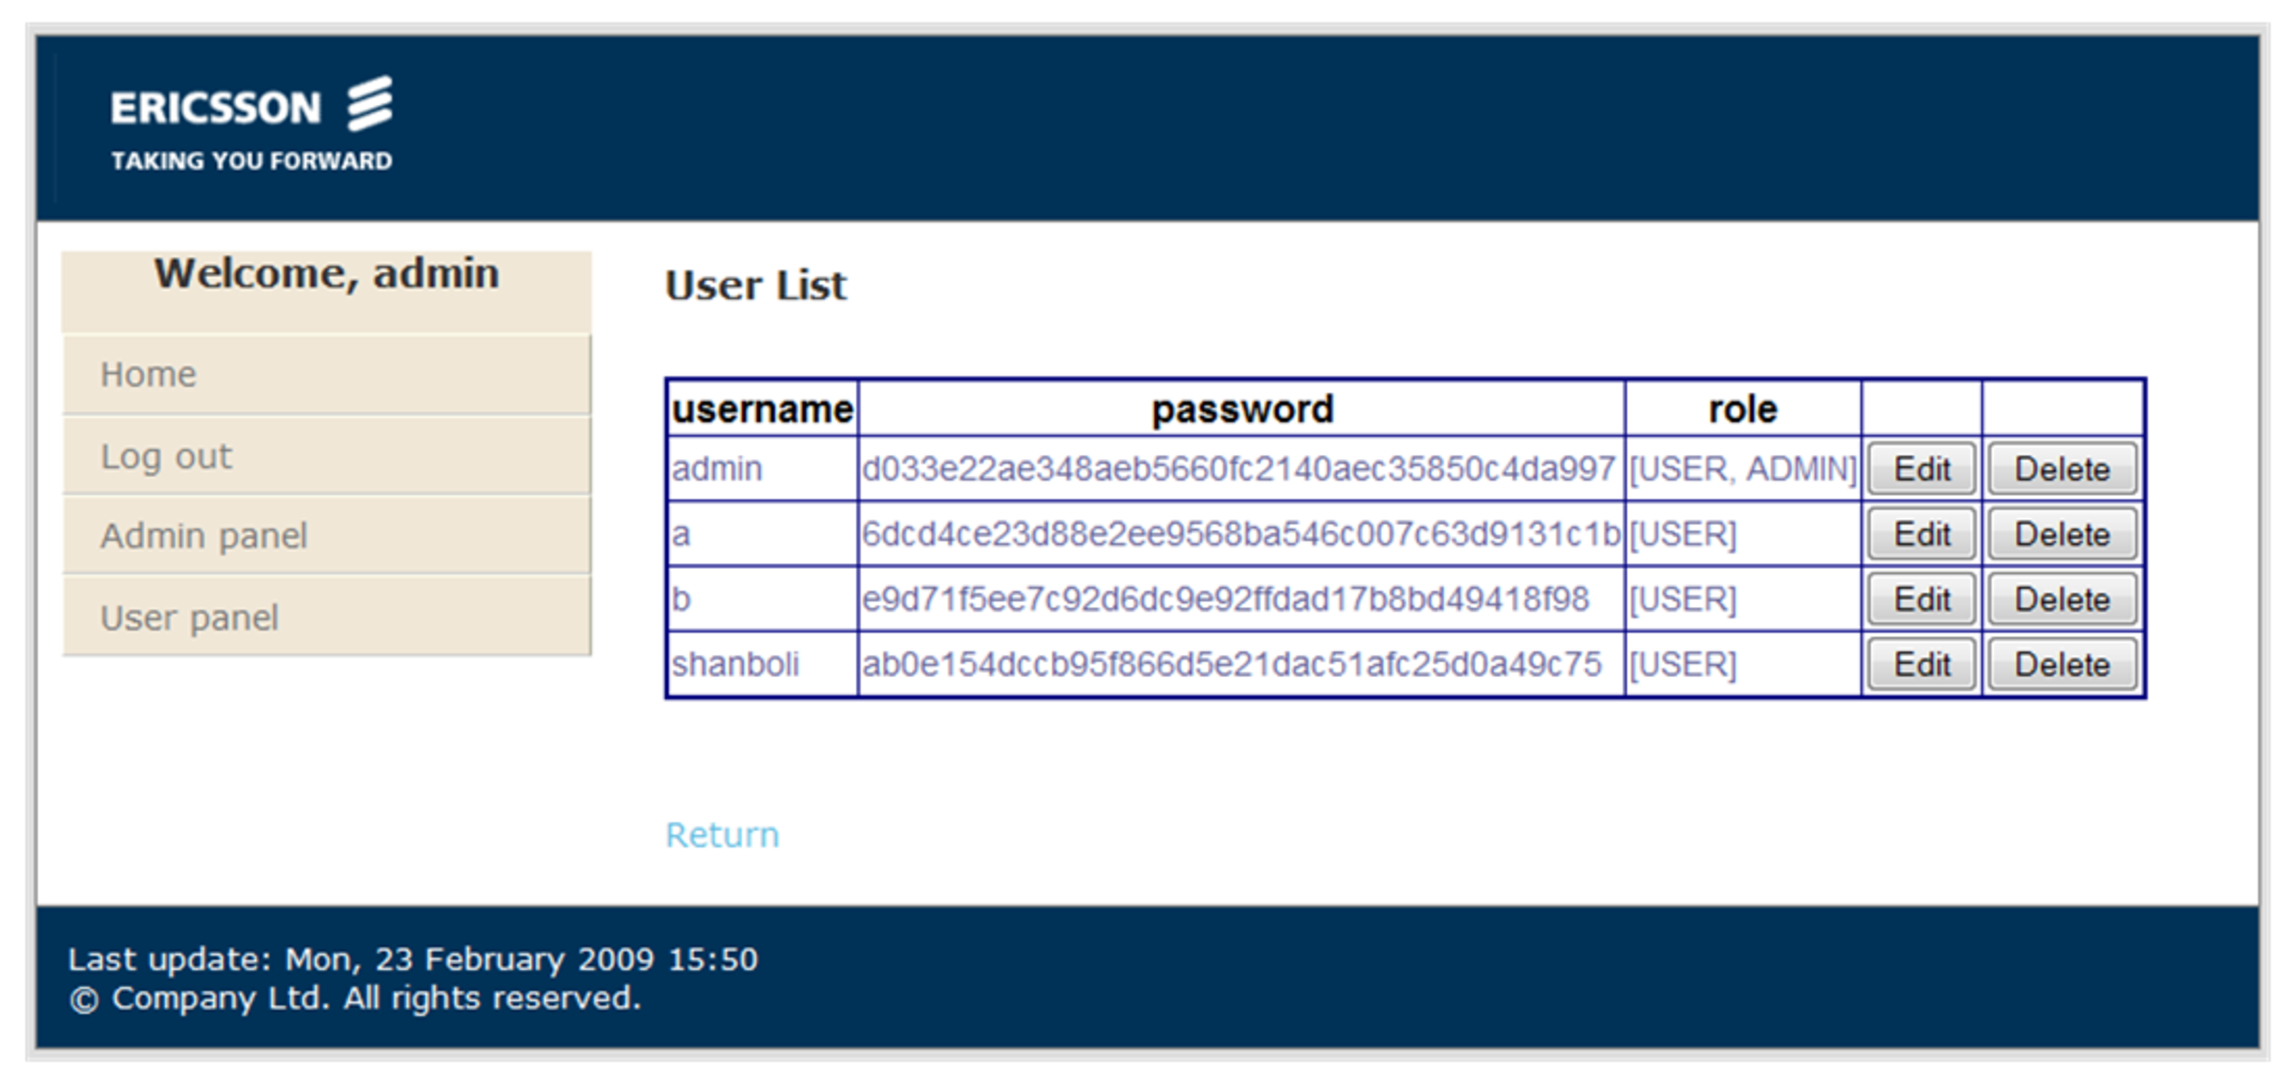
\epsfig{file=chap07/resources/user_list_desktop, width=5.2in}
\caption{User list of administrator panel}
\label{fig:UserListOfAdministratorPanel}
\end{figure} 

Figure \ref{fig:AdministratorViewOfUserInformation} shows a administrator view of user info. The administrator can update user's basic info, E.g. password and roles. Administrators can change SIP relevant information, such as user's phone number, user's contact list and user's VoIP account info by clicking ``show'' button in the SIP relevant info section.

\begin{figure}[!hbtp]
\centering
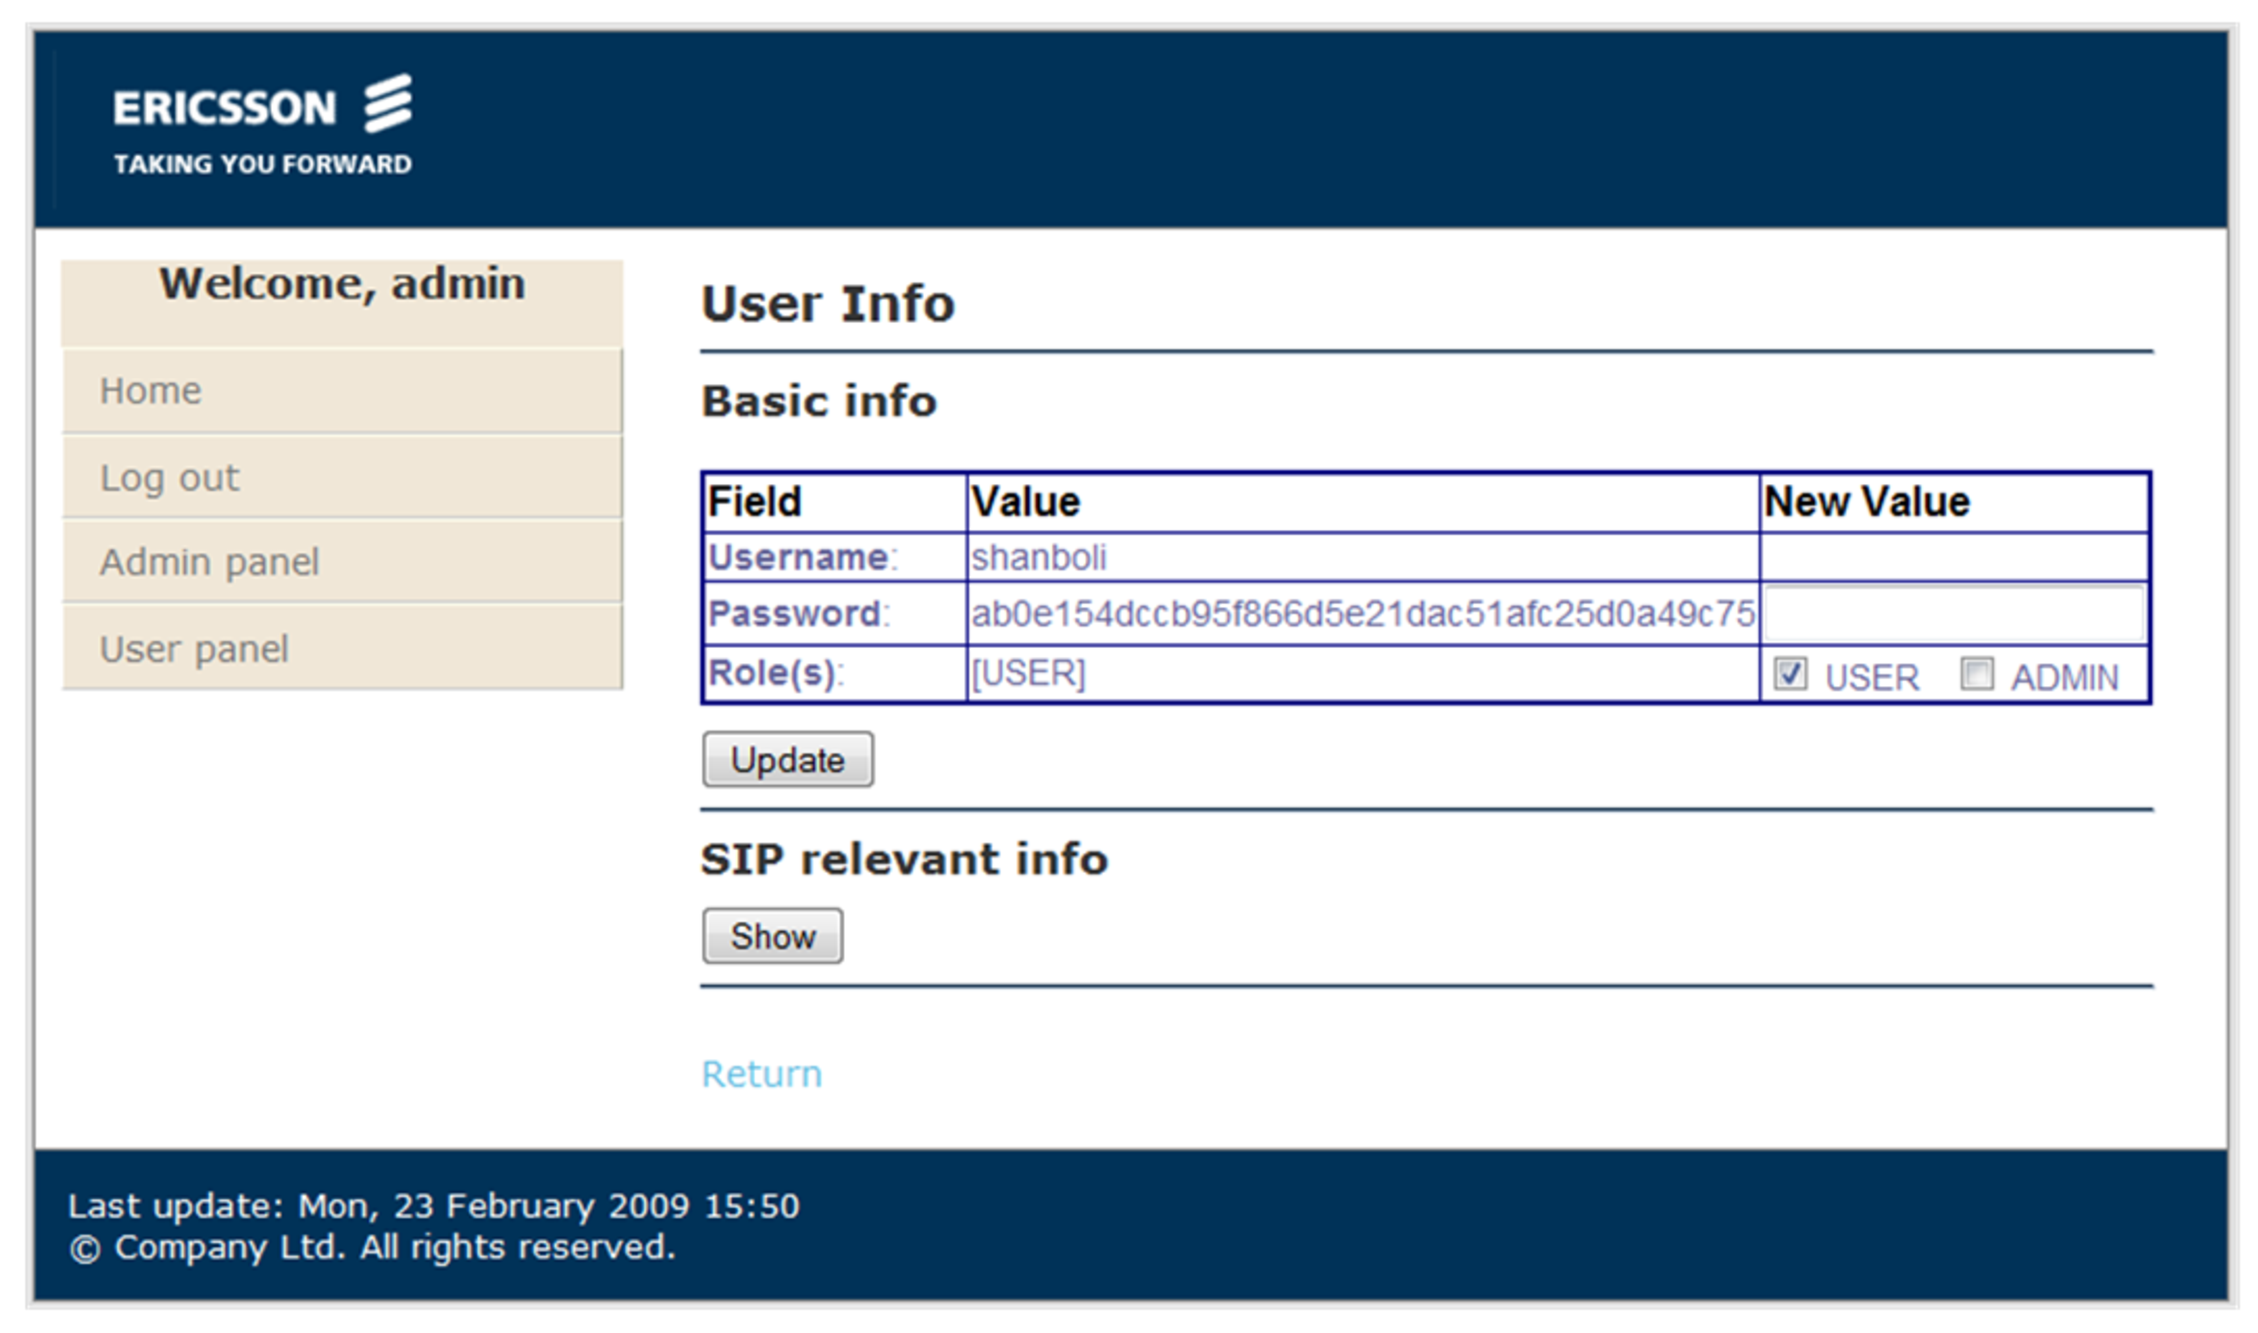
\epsfig{file=chap07/resources/admin_view_of_user_info, width=5.2in}
\caption{Administrator view of user information}
\label{fig:AdministratorViewOfUserInformation}
\end{figure} 

\section{Validation mechanism}
\label{sec:WebApplication:ValidationMechanism}

The validation of web application is implemented both at presentation tier and logic tier. On presentation tier, all form are validated by \texttt{javascript}. 

\subsection{Page level}
\label{sec:WebApplication:ValidationMechanism:PageLevel}

The validation on presentation layer can save the time of communication between browser and server. Web Call Example Application uses \texttt{JavaScript} to validate user input. All pages share the same generic validation methods. An example code of ``checking if a field is empty'' is shown in Listing \ref{JavaScriptValidationCode}.

\lstdefinelanguage{Java}
{morekeywords={function, alert, true, false, return}}
\lstset{language=Java}
\lstset{emph={function}, emphstyle={\color{blue}},
		  emph={value}, emphstyle={\color{purple}},}

\begin{lstlisting}[frame=lines, float=!bph, caption=JavaScript validation code, label=JavaScriptValidationCode]
function has_value(field, alert_message) {
    if (field.value == null || field.value == "") {
        alert(alert_message);
        return false;
    }
    return true;
}
\end{lstlisting}

\subsection{Server level}
\label{sec:WebApplication:ValidationMechanism:ServerLevel}

However, to prevent user disables \texttt{javascript}, there is also a validation mechanism on server side, that is called server level validation. To make the server response faster, only important or sensitive actions use a server level validation. E.g. The action of changing password has a server level validation of checking if password matched. The action of cancel call is another sensitive function. Beside the session id, server will also check if this session belongs to the user who want to cancel it. This will prevent from arbitrary interrupt calls.

\section{Session control}
\label{sec:WebApplication:SessionControl}

Web Call Example Application supports multi thread actions, that is many users can make phone calls concurrently. An \texttt{enum} class \texttt{CallSessions} works as a singleton\footnote{Singleton is a design pattern that used to restrict instantiation of a class to one object.} and manages call sessions. A class diagram of \texttt{CallSessions} is shown in Figure \ref{fig:ClassDiagramOfCallSessions}. It can be seen from picture, the four methods \texttt{add}, \texttt{getCallInfo}, \texttt{remove}, \texttt{contains} supply a very convenient way to manipulate sessions. A instance of \texttt{CallInfo} contains all of information of a phone call, it can be treated as a information pack.

\begin{figure}[!hbtp]
\centering
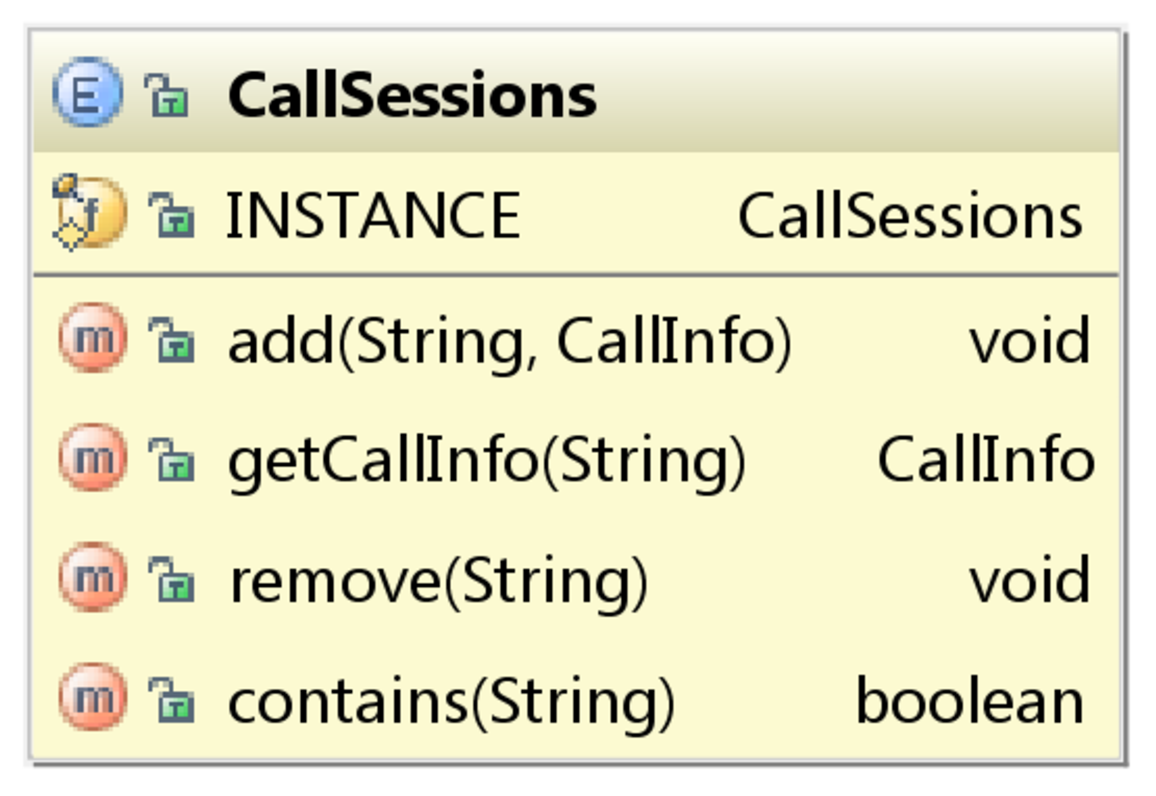
\epsfig{file=chap07/resources/CallSessions_class_diagram, width=2.5in}
\caption{Class diagram of CallSessions}
\label{fig:ClassDiagramOfCallSessions}
\end{figure} 

\section{Ajax in web application}
\label{sec:WebApplication:AjaxInWebApplication}

Ajax\label{sym:Ajax} is short for Asynchronous JavaScript and XML. It is a set of Internet techniques used on the client to generate interactive web applications or rich Internet applications. For more detail about Ajax, please refer to \textit{Ajax : A New Approach to Web Applications} by Jesse James Garrett\cite{Ajax}.

There are two places use Ajax in Web Call Example Application. One is at phone to phone call page, which is shown in Figure \ref{fig:PhoneToPhoneCall}. When user chooses a different VoIP service provider account. An Ajax request will be used to fetch account information from server. The fields will be updated automatically after browser get new account info. And there is no refresh of the page. 

\section{Java ME helper}
\label{sec:WebApplication:JavaMEHelper}

\section{Database}
\label{sec:WebApplication:Database}

\textsf{TODO: remember to write the first user will be administrator.}


\subsection{Design of database}
\label{sec:WebApplication:Database:DesignOfDatabase}

\subsection{User database utility}
\label{sec:WebApplication:Database:UserDatabaseUtility}

\section{Security}
\label{sec:WebApplication:Security}

\subsection{Certificate}
\label{sec:WebApplication:Security:Certificate}

\subsection{Security constraint}
\label{sec:WebApplication:Security:SecurityConstraint}

\subsection{Authorization}
\label{sec:WebApplication:Authorization}

% ********** End of chapter **********
